\documentclass[a4paper,UKenglish,cleveref, autoref, thm-restate]{oasics-v2021}
%This is a template for producing OASIcs articles. 
%See oasics-v2021-authors-guidelines.pdf for further information.
%for A4 paper format use option "a4paper", for US-letter use option "letterpaper"
%for british hyphenation rules use option "UKenglish", for american hyphenation rules use option "USenglish"
%for section-numbered lemmas etc., use "numberwithinsect"
%for enabling cleveref support, use "cleveref"
%for enabling autoref support, use "autoref"
%for anonymousing the authors (e.g. for double-blind review), add "anonymous"
%for enabling thm-restate support, use "thm-restate"
%for enabling a two-column layout for the author/affilation part (only applicable for > 6 authors), use "authorcolumns"
%for producing a PDF according the PDF/A standard, add "pdfa"
%
%\pdfoutput=1 %uncomment to ensure pdflatex processing (mandatatory e.g. to submit to arXiv)
%\hideOASIcs %uncomment to remove references to OASIcs series (logo, DOI, ...), e.g. when preparing a pre-final version to be uploaded to arXiv or another public repository
%
%\graphicspath{{./graphics/}}%helpful if your graphic files are in another directory
\usepackage{lmodern}
\usepackage{graphicx}
\usepackage{booktabs}
\usepackage{wrapstuff}
\usepackage{numprint}
\usepackage{wrapfig}
\usepackage{amsfonts}
\usepackage{mathpartir}
\usepackage{tikz}
\usepackage{mystyle}
\usepackage{upquote}
\bibliographystyle{plainurl}% the mandatory bibstyle

\definecolor{blue}{rgb}{0.38, 0.51, 0.71} %glaucous, 97,130,181, #6182B5
\definecolor{darkblue}{RGB}{17, 42, 60} % 112A3C
\definecolor{red}{RGB}{175, 49, 39} % AF3127
\definecolor{orange}{RGB}{217, 156, 55} % D99C37
\definecolor{green}{RGB}{144, 169, 84} % 90A954
\definecolor{palegreen}{RGB}{197, 184, 104} % C5B868
\definecolor{yellow}{RGB}{250, 199, 100} % FAC764
\definecolor{brokenwhite}{RGB}{218, 192, 166} % DAC0A6
\definecolor{brokengrey}{rgb}{0.77, 0.76, 0.82} % {196,194,209}, C4C2D1

\title{Isabelle/Solidity: A Tool  for the Verification of Solidity Smart Contracts (tool paper)} %TODO Please add

%\titlerunning{Dummy short title} %TODO optional, please use if title is longer than one line

\author{Asad {Ahmed}}{University of Exeter, Exeter EX4 4PY, UK \and \url{https://sites.google.com/view/asad-ahmed/home} }{a.ahmed6@exeter.ac.uk}{https://orcid.org/0000-0001-8276-0975}{}%TODO mandatory, please use full name; only 1 author per \author macro; first two parameters are mandatory, other parameters can be empty. Please provide at least the name of the affiliation and the country. The full address is optional. Use additional curly braces to indicate the correct name splitting when the last name consists of multiple name parts.

%\author{Joan R. Public\footnote{Optional footnote, e.g. to mark corresponding author}}{Department of Informatics, Dummy College, [optional: Address], Country}{joanrpublic@dummycollege.org}{[orcid]}{[funding]}
\author{Diego Marmsoler}{University of Exeter, Exeter EX4 4PY, UK}{d.marmsoler@exeter.ac.uk}{[https://orcid.org/0000-0003-2859-7673]}{}

\authorrunning{J. Open Access and J.\,R. Public} %TODO mandatory. First: Use abbreviated first/middle names. Second (only in severe cases): Use first author plus 'et al.'

\Copyright{Jane Open Access and Joan R. Public} %TODO mandatory, please use full first names. LIPIcs license is "CC-BY";  http://creativecommons.org/licenses/by/3.0/
%\ccsdesc[100]{\textcolor{red}{Replace ccsdesc macro with valid one}} %TODO mandatory: Please choose ACM 2012 classifications from https://dl.acm.org/ccs/ccs_flat.cfm 

\begin{CCSXML}
	<ccs2012>
	   <concept>
		   <concept_id>10002978.10002986.10002990</concept_id>
		   <concept_desc>Security and privacy~Logic and verification</concept_desc>
		   <concept_significance>500</concept_significance>
		   </concept>
	 </ccs2012>
\end{CCSXML}

\ccsdesc{Security and privacy~Logic and verification}

\keywords{Program Verification, Smart Contracts, Isabelle, Solidity} %TODO mandatory; please add comma-separated list of keywords

\category{} %optional, e.g. invited paper

\relatedversion{} %optional, e.g. full version hosted on arXiv, HAL, or other respository/website
%\relatedversiondetails[linktext={opt. text shown instead of the URL}, cite=DBLP:books/mk/GrayR93]{Classification (e.g. Full Version, Extended Version, Previous Version}{URL to related version} %linktext and cite are optional

%\supplement{}%optional, e.g. related research data, source code, ... hosted on a repository like zenodo, figshare, GitHub, ...
%\supplementdetails[linktext={opt. text shown instead of the URL}, cite=DBLP:books/mk/GrayR93, subcategory={Description, Subcategory}, swhid={Software Heritage Identifier}]{General Classification (e.g. Software, Dataset, Model, ...)}{URL to related version} %linktext, cite, and subcategory are optional

%\funding{(Optional) general funding statement \dots}%optional, to capture a funding statement, which applies to all authors. Please enter author specific funding statements as fifth argument of the \author macro.
\funding{This work was supported by the Engineering and Physical Sciences Research Council [grant number EP/X027619/1]}

\acknowledgements{I want to thank \dots}%optional

%\nolinenumbers %uncomment to disable line numbering

%Editor-only macros:: begin (do not touch as author)%%%%%%%%%%%%%%%%%%%%%%%%%%%%%%%%%%
\EventEditors{John Q. Open and Joan R. Access}
\EventNoEds{2}
\EventLongTitle{42nd Conference on Very Important Topics (CVIT 2016)}
\EventShortTitle{CVIT 2016}
\EventAcronym{CVIT}
\EventYear{2016}
\EventDate{December 24--27, 2016}
\EventLocation{Little Whinging, United Kingdom}
\EventLogo{}
\SeriesVolume{42}
\ArticleNo{23}
%%%%%%%%%%%%%%%%%%%%%%%%%%%%%%%%%%%%%%%%%%%%%%%%%%%%%%

\begin{document}

\maketitle

%TODO mandatory: add short abstract of the document
\begin{abstract}
	Smart contracts are an important innovation in Blockchain which allow to automate financial transactions.
	Every day, hundreds of thousands of new contracts are deployed managing millions of dollars' worth of transactions.
	Thus, bugs in smart contracts may lead to high financial losses and it is important to get them right before deploying them to the Blockchain.
	To address this problem we developed Isabelle/Solidity, a tool for the deductive verification of smart contracts in Isabelle.
	The tool is implemented as a definitional extension for the Isabelle proof assistant and thus complements existing tools in this area which are mostly based on axiomatic approaches.
	In this paper we describe Isabelle/Solidity and demonstrate it by verifying a casino contract from the VerifyThis long term verification challenge.
\end{abstract}

\section{Introduction}
\label{sec-intro}
One important innovation which comes with blockchain are so-called \emph{smart contracts}.
These are digital contracts which are automatically executed once certain conditions are met and which are used to automate transactions on the blockchain.
For instance, a payment for an item might be released instantly once the buyer and seller have met all specified parameters for a deal.
Every day, hundreds of thousands of new contracts are deployed~\cite{etherscan:contracts} managing millions of dollars' worth of transactions~\cite{ycharts:transactions}.\looseness-1
%Smart contracts are often used to automate financial transactions and thus they play a central role in the development of \emph{FinTech}, a technological revolution of the financial services sector.
%Therefore, they are of particular importance to the UK, where financial services are one of the largest industries contributing up to 9\% of the total economic output~\cite{Hutton2021}.

Technically, a smart contract is \emph{code which is deployed to a blockchain} and which can be executed by sending special transactions to it.
Thus, as for every computer program, smart contracts may contain bugs which can be exploited.
However, since smart contracts are often used to automate financial transactions, such exploits may result in huge economic losses.
%For example, in 2016 a vulnerability in an Ethereum smart contract was exploited resulting in a loss of approximately \$60M~\cite{Bahrynovska2017}.
%More recently, hackers had exploited a vulnerability in the DeFi-platform Poly Network to steal \$600M~\cite{BBC2021}.
%As another example, an incorrectly initialised contract was the root cause of the Parity Wallet bug that froze \$280M~\cite{perez.ea:smart:2021}.
In general, it is estimated that since 2019, more than \$5B was stolen due to vulnerabilities in smart contracts~\cite{CipherTrace2021}.
%In the healthcare sector, the impact of such vulnerabilities may be even worse since it may threaten the patients lifes.

The high impact of vulnerabilities in smart contracts together with the fact that once deployed to the blockchain, they cannot be updated or removed easily, makes it important to ``\emph{get them right}'' before they are deployed.
%Thus, companies have specialised to provide dedicated auditing services in which experts analyse smart contracts for vulnerabilities.
%Unfortunately, however, \highlight{even rigorous security audits cannot guarantee correctness of smart contracts} as shown in a more recent attack in which \$31M was stolen from a smart contract which had received already three security audits throughout the year~\cite{Goodin2021}.
To this end, we developed Isabelle/Solidity, a tool for the verification of Solidity smart contracts.
The main aim of this paper is to introduce the tool and demonstrate it in terms of an example.
To this end its contribution is two-fold:
\begin{itemize}
	\item We provide an overview of the technical architecture of Isabelle/Solidity.
	\item We use it to verify the casino contract from the VerifyThis verification challenge.
\end{itemize}

\section{Overview}
\label{sec-overview}

\autoref{fig:approach} depicts an overview of our approach to verify Solidity smart contract.
\begin{figure}[!h]
    \centering
    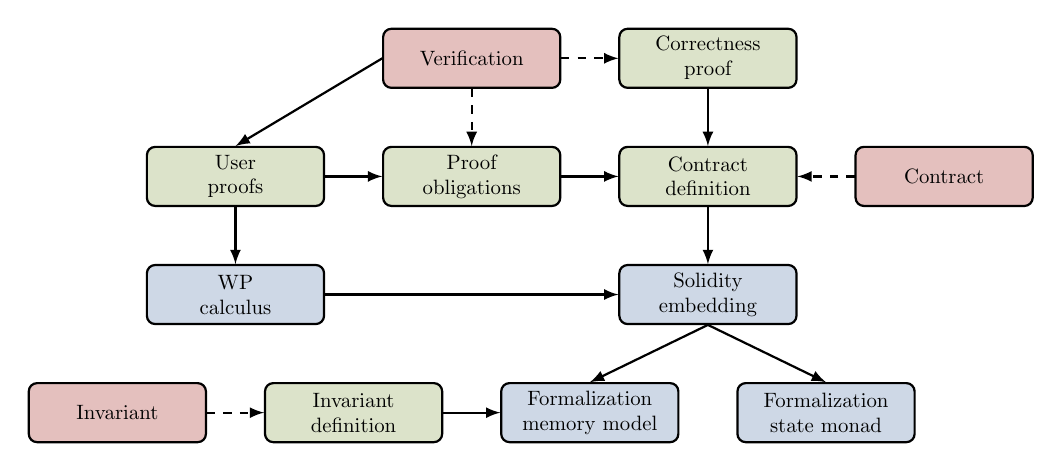
\begin{tikzpicture}[%
        thick,scale=0.75, every node/.style={scale=0.75},
        basic/.style ={rounded corners=3pt, draw, minimum width=3cm, minimum height=1cm, align=center},
        theory/.style={basic, fill=blue!95!black!30},
        temp/.style={basic, fill=green!95!black!30},
        feature/.style={basic, fill=red!95!black!30},
        dep/.style={-latex},
        gen/.style={-latex,dashed}
        ]
        \node[feature] (ver) at (0,0) {Verification};
        \node[temp] (obl) at (0,-2) {Proof \\ obligations};
        \node[temp] (usr) at (-4,-2) {User \\ proofs};
        \node[temp] (cor) at (4,0) {Correctness \\ proof};
        \node[temp] (cnt) at (4,-2) {Contract \\ definition};
        \node[feature] (spc) at (8,-2) {Contract};
        \node[theory] (wpc) at (-4,-4) {WP \\ calculus};
        \node[theory] (lan) at (4,-4) {Solidity \\ embedding};
        \node[feature] (isc) at (-6,-6) {Invariant};
        \node[temp] (idf) at (-2,-6) {Invariant \\ definition};
        \node[theory] (fmm) at (2,-6) {Formalization \\ memory model};
        \node[theory] (fsm) at (6,-6) {Formalization \\ state monad};
        \draw[dep] (ver.west) -- (usr.north);
        \draw[gen] (ver.south) -- (obl.north);
        \draw[gen] (ver.east) -- (cor.west);
        \draw[dep] (cor.south) -- (cnt.north);
        \draw[gen] (spc.west) -- (cnt.east);
        \draw[dep] (usr.south) -- (wpc.north);
        \draw[dep] (usr.east) -- (obl.west);
        \draw[dep] (obl.east) -- (cnt.west);
        \draw[dep] (cnt.south) -- (lan.north);
        \draw[dep] (wpc.east) -- (lan.west);
        \draw[dep] (lan.south) -- (fsm.north);
        \draw[dep] (lan.south) -- (fmm.north);
        \draw[dep] (idf.east) -- (fmm.west);
        \draw[gen] (isc.east) -- (idf.west);
    \end{tikzpicture}
    \caption{Isabelle/Solidity: theories (blue), commands (red), and generated artefacts (green). \label{fig:approach}}
\end{figure}
Isabelle/Solidity is based on four Isabelle theories which are represented by the {\color{blue}blue rectangles}:
\begin{description}
    \item[Formalization state monad]
    We model Solidity programs as functions which manipulate states.
    Such functions are usually described in terms of state monads~\cite{Wadler1993} and this theory contains our formalization of it based on \cite{Cock2008}.
    \item[Formalization memory model]
    Solidity has a quite particular memory model with different types of stores which support different types of data structures.
    This theory contains our formalization of the Solidity memory model.
    It also defines the notion of a Solidity state as a collection of different stores.
    \item[Solidity embedding]
    A Solidity statement is defined as a particular state monad manipulating a Solidity state.
    This theory contains definitions for all our Solidity statements.
    \item[WP calculus]
    To support a user in the verification of properties for our Solidity programms we provide a weakest precondition calculus~\cite{Dijkstra1975} for our Solidity statements.
    This theory formalizes the calculus.
\end{description}

In addition to the theories described above, Isabelle/Solidity extends the Isabelle proof assistant by means of three new definitional commands represented by the {\color{red}red rectangles} in \autoref{fig:approach}.
Each of the commands generates lower-level definitions and theorems for Isabelle/HOL which are represented as {\color{green}green rectangles}.
\begin{description}
    \item[Contract]
    This command allows a user to specify a new contract.
    It requires a user to specify a list of member variables, a constructor, and a list of methods.
    For each method the user can specify a list of parameters as well as a method body.
    The body is provided as a state monad using the monads defined in the corresponding Isabelle theory.
    The command then generates definitions for the \emph{contract's methods}.
    To this end each method is mapped to a corresponding partial function definition~\cite{Krauss2010}.
    \item[Invariant]
    This command supports a user in the specification of an invariant for the contract.
    An invariant is specified as a HOL formula over the store and balance of the contract.
    The command then uses the typing information of member variables to generates a corresponding \emph{invariant definition}.
    \item[Verification]
    This command triggers the verification of a contract.
    It requires a user to provide an invariant as well as postconditions for the methods.
    Then it presents the user with a list of \emph{proof obligations} for each of the contract's methods.
    The users then need to discharge these proof obligations by providing a corresponding \emph{proof}.
    To this end they can use the WP calculus provided by our framework.
    After discharging these obligations Isabelle/Solidity proves an overall \emph{correctness theorem} which guarantees that the invariant as well as postconditions are not violated.
\end{description}

\section{Case Study}
To demonstrate Isabelle/Solidity we use it to verify the casino contract from the VerifyThis long-term verification challenge~\cite{verifythis:casino}.
The version of the contract used here is provided in Appendix \ref{sec:app1}.
%
The casino contract implements a betting game based on guessing the outcome of coin-tossing.
%
At any time, the game is characterized by three states, i.e., \texttt{IDLE}, \texttt{GAME\_AVAILABLE} and \texttt{BET\_PLACED}.
%
Initially, the game is in the \texttt{IDLE} state.
%
The game has been implemented in Solidity using the following functions:
%
\begin{itemize}
\item The operator can create a new game by calling the \texttt{creatGame} function and provide the hash value of a secret number.
The function stores the secret number and changes the state to \texttt{GAME\_AVAILABLE}.
%
\item Once in state \texttt{GAME\_AVAILABLE}, a player can place a bet by invoking the \texttt{placeBet} function and provide a guess (\texttt{HEADS} or \texttt{TAILS}).
This function stores the player's address, its guess, and the amount of the bet, and changes the state to \texttt{BET\_PLACED}.
%
\item Now, the operator can decide the bet anytime by calling the \texttt{decideBet} function and providing the secret number.
The secret number is then used to decide the outcome of the coin tossing (\texttt{HEADS} or \texttt{TAILS}).
If the player's guess is correct, the double of the amount of the bet is transferred to their address.
Otherwise, the amount equal to the bet is added to the pot.
The function also changes the state of the game to \texttt{IDLE}.
%
\item The operator may add money to the bet, at anytime, using \texttt{addToPot} but can only remove money if the game is in not in state \texttt{BET\_PLACED} by calling \texttt{removeFromPot}.
\end{itemize}
%
%%THIS CAN MOVE UP IN THE INTRODUCTION
%The casino smart contract was selected for two reasons:
%First, it makes use of advanced features of Solidity including advanced data types, global and local variables, functions, modifiers. 
%Thus, it requires to develop powerful equivalent syntax support in the proposed tool to embed the program logic.
%Two, from verification aspect, casino has been employed as a case study in literature and hence allows to compare and report the result to gauge the performance of the proposed tool, comparatively.
%
\section{Specification}
To verify a smart contract in Isabelle/Solidity we first need to specify it.
To this end Isabelle/Solidity provides the \texttt{\color{isacom}contract} command which supports a user in this task.
The command requires a user to specify a list of member variables and corresponding types, followed by a specification of the constructor and the contract's methods.

\paragraph*{Storage Variables}
Listing \ref{fig:isadt} shows the specification of storage variables for the casino smart in Isabelle/Solidity.
\begin{code}{label={fig:isadt}}{isabelle}{Isabelle/Solidity data types for Casino}
contract Casino
  for state: StateT
  and operator: AddressT
  and player: AddressT
  and pot: IntT
  and hashedNumber: BytesT
  and bet: IntT
  and guess: CoinT
\end{code}
Isabelle/Solidity supports most of the basic Solidity data types, such as bit-sized integers, bytes, and addresses.
Enums can be encoded as integers with corresponding abbreviations.
%
\paragraph*{Methods}
We do not show the specification for all of the methods of the casino contract here but we only discuss one.
The others can be similarly translated from the original Solidity contract.

The specification of a new method can be done using the keyword \texttt{\color{isargreen}emethod}.
To allow a method to receive funds we can set the payable flag by using the corresponding \texttt{\color{isargreen}payable} keyword.
What follows is a specification of stack (\texttt{\color{isargreen}param}), memory (\texttt{\color{isargreen}memory}), and calldata (\texttt{\color{isargreen}calldata}) parameters and corresponding types.
Finally, one can provide the body of the function using the \texttt{\color{isargreen}where} keyword followed by a corresponding monad specification (using \texttt{"\texttt{\color{isarlight}do} \{\dots\}",} notation).

Listing \ref{fig:isamethod} shows the specification of the function \texttt{decideBet}.
\begin{code}{label={fig:isamethod}}{isabelle}{Isabelle/Solidity method for Casino}
emethod decideBet payable
  param secretNumber: IntT
where
  do {
    byOperator;
    inState (Sint BET_PLACED);
    $\langle$assert$\rangle$ (hashedNumber $\sim\textsubscript{s}$ [] $\langle$=$\rangle$ ($\langle$keccak256$\rangle$ (secretNumber $\sim$ [])));
    decl TSint secret;
    secret [] ::= IF ((secretNumber $\sim$ []) $\langle\%\rangle$ $\langle$sint$\rangle$ 2) $\langle$=$\rangle$ ($\langle$sint$\rangle$ 0) 
    				        THEN $\langle$sint$\rangle$ HEADS ELSE $\langle$sint$\rangle$ TAILS;
    IF (secret $\sim$ []) $\langle$=$\rangle$(guess $\sim\textsubscript{s}$ []) THEN
    do {
      decl TSint bet_old;
      bet_old [] ::= bet $\sim\textsubscript{s}$ [];
      bet [] ::=$\textsubscript{s}$ $\langle$sint$\rangle$ 0;
      pot [] ::=$\textsubscript{s}$ ((pot $\sim\textsubscript{s}$ []) $\langle$-$\rangle$ (bet_old $\sim$ []));
      $\langle$transfer$\rangle$ (player $\sim\textsubscript{s}$ []) ((bet $\sim\textsubscript{s}$ []) $\langle$*$\rangle$ ($\langle$sint$\rangle$ 2))
    }
    ELSE
    do {
      pot [] ::=$\textsubscript{s}$ pot $\sim\textsubscript{s}$ [] $\langle$+$\rangle$ bet $\sim\textsubscript{s}$ [];
      bet [] ::=$\textsubscript{s}$ $\langle$sint$\rangle$ 0
    };
    state [] ::=$\textsubscript{s}$ $\langle$sint$\rangle$ IDLE
  },
\end{code}
It is declared to be payable and accepts one parameter \texttt{secretNumber}, of integer type.
Lines 5-7, implement preconditions for deciding a bet, i.e., only the operator can call the function, the game should be in state \texttt{BET\_PLACED} and \texttt{secretNumber} should be equal to the \texttt{hashedNumber}. 
For this purpose, Isabelle/Solidity employs \texttt{\color{isarblue}{assert}} which models the Solidity \texttt{\color{blue}{require}} command. 

Isabelle/Solidity also supports other Solidity statements, such as control structures and assignment operators.
For example, in Line 9, \texttt{\color{isarblue}{IF}}\dots \texttt{\color{isarblue}{THEN}}\dots \texttt{\color{isarblue}{ELSE}} reveals \texttt{HEADS} or \texttt{TAILS} by taking the modulus (\texttt{$\langle\%\rangle$}) of \texttt{secretNumber}. 
For assignment operators, Isabelle/Solidity distinguishes between stack (\texttt{::=}) and storage (\texttt{::=}$\textsubscript{s}$) assignments along with corresponding lookup operators ($\sim$ and $\sim\textsubscript{s}$). 
%

%
%Next, 
%%
%in Line 10 (of Listing \ref{fig:isamethod}), \texttt{transfer\_monad} transfers (special function) an amount  equal to the bet is transferred to the operator account.
%

%
%
\section{Verification}
%
%
%
Isabelle/Solidity facilitates the specification of invariants using the \texttt{\color{isarblue}invariant} command.
This command requires a user to provide the name of the invariant, followed by the invariant as predicates formulated over the contract's store and balance.
It then generates a definition for the invariant which, in addition to the predicate specified by the user, also requires the value of member variables to adhere to their types.
The command also proves corresponding a introduction and elimination rules which can be invoked for automated verification of the invariants.

\begin{Example}{Invariant}{invariant}
	Assume that we want to ensure our contract has always enough funds to cover the payout of players.
  More formally, we want to ensure that, whenever the game is in the \texttt{BET\_PLACED} state, the contract's internal balance satisfies:
	\begin{equation}
	  pot\_balance(s, b)=b \ge s(\STR{pot}) + s(\STR{bet})~\wedge~s(\STR{bet}) \leq s(\STR{pot})
	\end{equation}\label{eq:inv}
  and if it is not in \texttt{BET\_PLACED}, then 
  \begin{equation}
		pot\_balance(s, b)=b \ge pot 
  \end{equation}\label{eq:inv1}
%
The corresponding specification in Isabelle/Solidity is given in Listing \ref{def:inv}.
\begin{code}{label={def:inv}}{isabelle}{Invariant in Isabelle/Solidity}
invariant pot_balance sb where
  (fst sb state = sdata.Value (Sint BET_PLACED)
    $\longrightarrow$ snd sb $\geq$ unat (valtype.sint (sdata.vt pot)) 
	                + unat (valtype.sint (sdata.vt bet))
        $\wedge$ valtype.sint (sdata.vt bet) $\leq$ valtype.sint (sdata.vt pot)) $\wedge$
  (fst sb state $\neq$ sdata.Value (Sint BET_PLACED)
    $\longrightarrow$  snd sb $\geq$ unat (valtype.sint (sdata.vt pot)))
  for "casino"
\end{code}
\end{Example}
%

%
To formally verify the invariant, Isabelle/Solidity provides the \texttt{\color{isarblue}verification} command. 
%
It requires the user to provide a name followed by an invariant specified using the invariant keyword.
Moreover, a user can provide postconditions for the constructor and each of the contract's methods.
The corresponding specification for our casino contract is shown in Listing \ref{def:ver}.
The postconditions require a method to update the corresponding state of the game properly.

\begin{code}{label={def:ver}}{isabelle}{Verification in Isabelle/Solidity}
verification pot_balance:
   pot_balance
  "K (K (K True))"
  "createGame" "createGame_post" and
  "placeBet" "placeBet_post" and
  "decideBet" "decideBet_post" and
  "addToPot" "K (K (K True))" and
  "removeFromPot" "K (K (K (K True)))"
  for "casino"
\end{code}
%\vskip
%\paragraph*{Discussions}
In order to automate the verification task, Isabelle/Solidity provides proof automation support in terms of a weakest precondition calculus.
Verification of the Casino smart contract using Isabelle/Solidity resulted in the exploration of a major vulnerability, i.e., Reenetrancy.
%
While verifying the invariant in Example \autoref{ex:invariant},  it was not possible to verify unless changing the order of the Line 32 and 33 (see Appendix \ref{sec:app1}) which enabled the completion of the verification task. 
%
It is due to possibility of calling the function \texttt{decideBet} without setting \texttt{bet}=\texttt{0} which may lead to unintended behaviour.  
%

\section{Related Work}
%
Considering the mission-critical nature of the smart contracts in blockchain technology, formal methods techniques, e.g., Model Checking \cite{antonino2020formalising}, theorem proving \cite{bhargavan2016formal}, have been employed to formally specify and verify Solidity smart contracts. Model checking \cite{clarke1997model}is a push-button automatic formal methods technique, however, has limited expressiveness due to finite-state machine modelling and is prone to state-space explosion. On the other hand, theorem proving is highly-expressive and has also been utilized for the verification of Solidity smart contracts. 

In theorem proving literature, deep and shallow embedding are two common approaches for the verification of Solidity language. A deep embedding of operational semantic of Solidity in SolidiKeY \cite{ahrendt2020functional} allows to formally specify and verify smart contracts using KeY theorem prover. Similarly, Jakab \cite{zakrzewski2018towards} formalizes a Coq interpreter, utilizing deep embedding of operational semantic of Solidity, for the smart contract verification. However, aforementioned works rely on the axiomatic verification approach therefore may lead to miss corner cases in verifying smart contracts. In this direction, Diego et al. \cite{marmsoler2022isabelle}  developed a deep embedding framework for denotational semantic of Solidity in Isabelle/HOL which support correct-by-construction approach for the formal verification of smart contracts. On the other hand, there are two notable efforts for shallow embedding of Solidity in Isabelle theorem prover. Ribeiro et al. \cite{ribeiro2020formal} utilize mix of deep and shallow embedding to develop an intermediary low-level specification language, \texttt{SOLI}, for the specification and verification of Solidity smart contracts in Isabelle/HOL. Whereas \cite{marmsoler2024secure} provides a shallow embedding of operational semantic of Solidity in Isabelle/HOL. The framework is equipped with complex data types, such as mappings and arrays and verification of invariants as compared to SOLI.

Isabelle/Solidity tool, proposed in this paper, is based on the shallow embedding approach \cite{marmsoler2024secure}. 
This is mainly due to the scope of the proposed tool.
% 
 %
The objective of the proposed tool is to formally specify and verify the correctness of the Solidity smart contracts which is best served, in terms of effort and time, by shallow embedding as compare to deep embedding. This has been empirically shown in \cite{marmsoler2024secure}.
%Considering the mission-critical nature of the smart contracts in blockchain technology, various formal methods techniques, such as Model Checking, theorem proving and SMT solvers, have been employed to formally specify and verify Solidity smart contracts. 
%%
%Solidifier \cite{antonino2020formalising}, VeriSol\footnote{\url{https://github.com/Microsoft/verisol}} and solc-verify \cite{hajdu2020solc} translates a given smart contract into equivalent Boogie script, an intermediate verification language, which is then employed for formal verification using bounded model checking and SMT solvers.
%%
%Model checking is a push-button automatic  formal methods technique, however, has limited expressiveness due to finite-state machine modelling and is prone to state-space explosion.
%%
%
%%
%Theorem proving is highly-expressive formal methods technique and has also been employed to formally specify and verify Solidity smart contracts. 
%%
%SolidiKeY \cite{ahrendt2020functional} accomplishes the task of verification using KeY theorem prover for a given smart contract specified as a dynamic logic (DL) formula. 
%%
%An intermediary low-level specification language, \texttt{SOLI} \cite{ribeiro2020formal}, allows to formally specify and verify smart contracts in Isabelle/HOL (\textcolor{red}{I doubt if it is axiomatic approach for Solidity smart contracts, need your comments}). 
%%Jackob  has proposed an interpreter in Coq theorem prover for Solidity using big-step semantic approach. 
%%
%%These efforts allow to formally specify and verify the Solidity smart contracts deductively using native proof theories in corresponding theorem provers. 
%%
%The above-mentioned research work  is based on axiomatic approach, thus, limits  verification capabilities of Solidity smart contracts. 
%%
%To overcome this issue, correct by construction approach has also been employed to formally specify and verify smart contracts.
%%
%Particularly, deep \cite{marmsoler2022isabelle} and shallow embedding \cite{marmsoler2024secure} of Solidity in Isabelle/HOL facilitate formal specification and verification of Solidity smart contracts.
%%
%Also we follow a definitional approach meaning that we generate lower level definitions from higher level domain constructs which ensures consistency by construction.
% %Particularly, deep embedding of Solidity statements as a datatype in Isabelle/HOL \cite{marmsoler2022isabelle} facilitates deductive reasoning about the language itself which in turn allows to formally specify and verify complex properties of Solidity smart contracts. 
%%
%%
%%
%%On the other hand, Isabelle/Solidity \cite{marmsoler2024secure} leverages upon the shallow embedding of Solidity in Isabelle/HOL in order to reduce the signification effort for verifying smart contracts with deep embedding approach.
%%
%
%%
% Isabelle/Solidity tool, proposed in this paper, is based on the shallow embedding approach \cite{marmsoler2024secure}. 
%% 
% Although, deep embedding furnishes deductive reasoning about the Solidity language itself but results in a significant effort to develop full support for the purpose.  
%%
%On the other hand, shallow embedding approach  offers  
%%
%%Also we follow a definitional approach meaning that we generate lower level definitions from higher level domain constructs which ensures consistency by construction.
%%

\section{Conclusion}
%%
%% Bibliography
%%
%
In this paper, we present Isabelle/Solidity tool for the formal specification and verification of Solidity smart contracts. 
%
The tool facilitates Solidity data-types, functions, modifiers, statements, expressions and post/pre-condition specifiers in Isabelle/HOL.
%
%
The formal specification relies upon the underlying shallow embedding of Solidity expressions and statements as state-monads and storage models for different types of stores in Solidity.
%
For the verification purpose, tool supports invariant specification for the contract that in turn is supported by verification condition generator to automate the verification process.
%
Finally, we evaluated the approach by means of the Casino case study.
%
The use of the Isabelle/Solidity resulted in the exploration of re-entrancy vulnerability in the original version of Casino smart contract.
%
However, there are few  challenges in order to  fully cover the advanced features of Solidity. 
%

%
In this regard, inheritance is one of the most notable Solidity feature which can be introduced in the proposed tool for verifying interesting properties of the smart contracts.
%
Moreover, from the verification point-of-view, automation can be further improved by providing specialized rules w.r.t the context of the smart contracts.


%
%% Please use bibtex, 
%\nocite{*}
\bibliography{oasics-v2021-sample-article}

\appendix

\section{Casino: Solidity Smart Contract}\label{sec:app1}


\begin{code}{label={fig:casino}}{solidity}{Solidity source code for the Casino}
	contract Casino {
		enum Coin { HEADS, TAILS } ;
		enum State { IDLE, GAME_AVAILABLE,  BET_PLACED }
		State private state; 
		address public operator, player;
		uint public pot;
		bytes32 public hashedNumber;
		uint public bet;
		Coin guess;

		function createGame(bytes32 hashNum) 
			public byOperator, inState(IDLE) { 
			hashedNumber = hashNum; 
			state = GAME_AVAILABLE;
		}

		function placeBet(Coin _guess) public payable inState(GAME_AVAILABLE) {
			require (msg.sender != operator);
			require (msg.value <= pot);
			state = BET_PLACED; 
			player = msg.sender; 
			bet = msg.value; 
			guess = _guess; 
		}

 		function decideBet(uint secretNumber) 
		public byOperator, inState(BET_PLACED) { 
			require (hashedNumber == keccak256(secretNumber)); 
			Coin secret = (secretNumber % 2 == 0)? HEADS : TAILS;
			if (secret == guess) {
				pot = pot - bet;  
				player.transfer(bet*2);  
				bet = 0;} 
			else {
				pot = pot + bet; 
				bet = 0;
				}
			state = IDLE;}
		function addToPot() public payable byOperator { pot = pot + msg.value;}

		function removeFromPot(uint amount) public byOperator, noActiveBet { 
			operator.transfer(amount);  
			pot = pot - amount;}
		}
\end{code}


%\cref{testenv-proposition} and \autoref{testenv-proposition} ...
%
%\section{Theorem-like environments}\label{sec:theorem-environments}
%
%List of different predefined enumeration styles:
%
%\begin{theorem}\label{testenv-theorem}
%Fusce eu leo nisi. Cras eget orci neque, eleifend dapibus felis. Duis et leo dui. Nam vulputate, velit et laoreet porttitor, quam arcu facilisis dui, sed malesuada risus massa sit amet neque.
%\end{theorem}
%
%\begin{lemma}\label{testenv-lemma}
%Fusce eu leo nisi. Cras eget orci neque, eleifend dapibus felis. Duis et leo dui. Nam vulputate, velit et laoreet porttitor, quam arcu facilisis dui, sed malesuada risus massa sit amet neque.
%\end{lemma}
%
%\begin{corollary}\label{testenv-corollary}
%Fusce eu leo nisi. Cras eget orci neque, eleifend dapibus felis. Duis et leo dui. Nam vulputate, velit et laoreet porttitor, quam arcu facilisis dui, sed malesuada risus massa sit amet neque.
%\end{corollary}
%
%\begin{proposition}\label{testenv-proposition}
%Fusce eu leo nisi. Cras eget orci neque, eleifend dapibus felis. Duis et leo dui. Nam vulputate, velit et laoreet porttitor, quam arcu facilisis dui, sed malesuada risus massa sit amet neque.
%\end{proposition}
%
%\begin{conjecture}\label{testenv-conjecture}
%Fusce eu leo nisi. Cras eget orci neque, eleifend dapibus felis. Duis et leo dui. Nam vulputate, velit et laoreet porttitor, quam arcu facilisis dui, sed malesuada risus massa sit amet neque.
%\end{conjecture}
%
%\begin{observation}\label{testenv-observation}
%Fusce eu leo nisi. Cras eget orci neque, eleifend dapibus felis. Duis et leo dui. Nam vulputate, velit et laoreet porttitor, quam arcu facilisis dui, sed malesuada risus massa sit amet neque.
%\end{observation}
%
%\begin{exercise}\label{testenv-exercise}
%Fusce eu leo nisi. Cras eget orci neque, eleifend dapibus felis. Duis et leo dui. Nam vulputate, velit et laoreet porttitor, quam arcu facilisis dui, sed malesuada risus massa sit amet neque.
%\end{exercise}
%
%\begin{definition}\label{testenv-definition}
%Fusce eu leo nisi. Cras eget orci neque, eleifend dapibus felis. Duis et leo dui. Nam vulputate, velit et laoreet porttitor, quam arcu facilisis dui, sed malesuada risus massa sit amet neque.
%\end{definition}
%
%\begin{example}\label{testenv-example}
%Fusce eu leo nisi. Cras eget orci neque, eleifend dapibus felis. Duis et leo dui. Nam vulputate, velit et laoreet porttitor, quam arcu facilisis dui, sed malesuada risus massa sit amet neque.
%\end{example}
%
%\begin{note}\label{testenv-note}
%Fusce eu leo nisi. Cras eget orci neque, eleifend dapibus felis. Duis et leo dui. Nam vulputate, velit et laoreet porttitor, quam arcu facilisis dui, sed malesuada risus massa sit amet neque.
%\end{note}
%
%\begin{note*}
%Fusce eu leo nisi. Cras eget orci neque, eleifend dapibus felis. Duis et leo dui. Nam vulputate, velit et laoreet porttitor, quam arcu facilisis dui, sed malesuada risus massa sit amet neque.
%\end{note*}
%
%\begin{remark}\label{testenv-remark}
%Fusce eu leo nisi. Cras eget orci neque, eleifend dapibus felis. Duis et leo dui. Nam vulputate, velit et laoreet porttitor, quam arcu facilisis dui, sed malesuada risus massa sit amet neque.
%\end{remark}
%
%\begin{remark*}
%Fusce eu leo nisi. Cras eget orci neque, eleifend dapibus felis. Duis et leo dui. Nam vulputate, velit et laoreet porttitor, quam arcu facilisis dui, sed malesuada risus massa sit amet neque.
%\end{remark*}
%
%\begin{claim}\label{testenv-claim}
%Fusce eu leo nisi. Cras eget orci neque, eleifend dapibus felis. Duis et leo dui. Nam vulputate, velit et laoreet porttitor, quam arcu facilisis dui, sed malesuada risus massa sit amet neque.
%\end{claim}
%
%\begin{claim*}\label{testenv-claim2}
%Fusce eu leo nisi. Cras eget orci neque, eleifend dapibus felis. Duis et leo dui. Nam vulputate, velit et laoreet porttitor, quam arcu facilisis dui, sed malesuada risus massa sit amet neque.
%\end{claim*}
%
%\begin{proof}
%Fusce eu leo nisi. Cras eget orci neque, eleifend dapibus felis. Duis et leo dui. Nam vulputate, velit et laoreet porttitor, quam arcu facilisis dui, sed malesuada risus massa sit amet neque.
%\end{proof}
%
%\begin{claimproof}
%Fusce eu leo nisi. Cras eget orci neque, eleifend dapibus felis. Duis et leo dui. Nam vulputate, velit et laoreet porttitor, quam arcu facilisis dui, sed malesuada risus massa sit amet neque.
%\end{claimproof}

\end{document}
